%% We use `subfiles' package
\documentclass[preamble.tex]{subfiles}
\begin{document}


\clearpage

\chapter{Results}
\label{ch:results}


\section{QuickHull}
\label{sec:quickhull}

Throughout this chapter we will use a \name{Data Parallel Haskell} implementation of the QuickHull algorithm that computes the convex hull of a finite set of points in the plane. It derives its name from the QuickSort algorithm and similarly uses a divide and conquer approach.

The convex hull for a set of points in the plane can be visualised as a polygon formed by a rubber band stretched around the points. The smallest set of points forming the polygon that encloses all other points is called the convex hull.

The result of finding convex hull of a set of points can be seen on the right of Figure~\ref{fig:qh-result}. The same figure depicts the three steps of the sample run of QuickHull algorithm.


\subsection{QuickHull in \DPH}

The \DPH implementation of QuickHull closely follows the recursive solution:
\begin{enumerate}
  \item Finds the points with smallest and largest $x$ coordinates (lines 12 and 13 and Figure~\ref{fig:qh-result} left). These points are bound to be in the convex hull.

  \item The line between the two points forms two subsets of points, which will be processed recursively (line 8) by @QuickHullR@ function.

  \item The recursive @QuickHullR@ function, given a subset of points and a line, determines the point, on one side of the line, @far@thest from it (line 27). This point is also in the convex hull.

  \item @QuickHullR@ also filters out all points on the other side of the line (line 25), keeping only the points @above@ the line.

  \item The two ends of the line each form a new line with the @far@ point to be recursively processed (line 19).

  \item The previous three steps are repeated expanding the convex hull until no more points are left above any of the lines. The recursion has finished and the points forming the lines constitute the convex hull.
\end{enumerate}


\begin{figure}
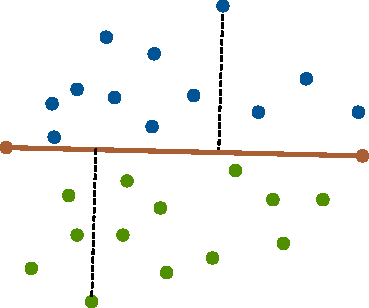
\includegraphics[width=0.3\textwidth]{img/Example-QuickHull-step1}~~~~~%
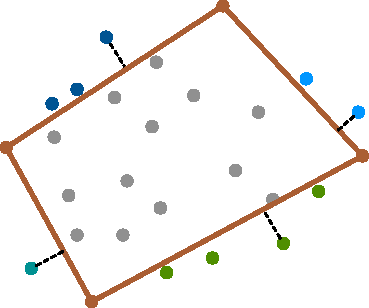
\includegraphics[width=0.3\textwidth]{img/Example-QuickHull-step2}~~~~~%
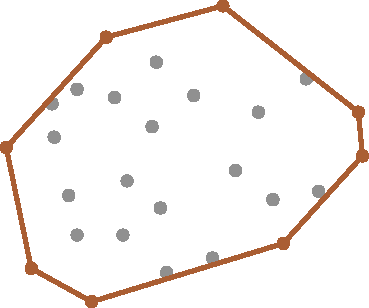
\includegraphics[width=0.3\textwidth]{img/Example-QuickHull-step3}%
\caption{Three steps of a sample run of data parallel QuickHull algorithm.}
\label{fig:qh-result}
\end{figure}


\begin{hscode}[%
  caption={\label{fig:dph-qh}\name{Data Parallel Haskell} implementation of QuickHull.},
  numbers=left,
]
type Point = (Double, Double)
type Line  = (Point,  Point)

quickHull :: [:Point:] -> [:Point:]
quickHull points
  | lengthP points == 0 = points
  | otherwise
  = concatP [: quickHullR points ends
                 | ends <- [: (minx, maxx), (maxx, minx) :] :]
  where
    xs   = [: x | (x, y) <- points :]
    minx = points !: minIndexP xs
    maxx = points !: maxIndexP xs

quickHullR :: [:Point:] -> Line -> [:Point:]
quickHullR points line@(start, end)
  | lengthP above == 0 = [:start:]
  | otherwise
  = concatP [: quickHullR above ends
                 | ends <- [:(start, far), (far, end):] :]
  where
    -- Find relative distance from each point to the line
    distances = [: distance p line | p <- points :]
    -- Only keep points above the line
    above = [: p | (p,c) <- zipP points distances, c > 0.0 :]
    -- Find the point farthest from the line
    far = points !: maxIndexP distances

-- Cross product used as distance-like measure
distance :: Point -> Line -> Double
distance (xo, yo) ((x1, y1), (x2, y2))
  = (x1 - xo) * (y2 - yo) - (y1 - yo) * (x2 - xo)
\end{hscode}



\subsection{QuickHull vectorisation}

The QuickHull program presented is a typical example of a divide and conquer algorithm. Recursive calls of @quickHullR@ function in most languages would be processed sequentially one at a time. However, in \DPH, the function is vectorised as described in Section~\ref{sec:Vectorisation} to give @quickHullR^@ of the following type:


\begin{hscode}[literate={^}{{$^\uparrow$}}1,]
-- Original
quickHullR  :: [:Point:] -> Line -> [:Point:]
-- Vectorised
quickHullR^ :: [:[:Point:]:] -> [:Line:] -> [:[:Point:]:]
\end{hscode}


The vectorised function is able to process not one, but an array of lines at a time. This means that the ``expansion'' of convex hull in every direction happens in one call of @quickHullR^@. In fact the three steps of vectorised QuickHull depicted in Figure~\ref{fig:qh-result} faithfully represent the only three calls to @quickHullR^@ required to find the convex hull.



\subsection{QuickHull in the backend}

The vectorised @quickHullR^@ function takes a \*nested parallel array* of points @[:[:Point:]:]@ as its first argument. It was discussed in Section~\ref{sec:Flattening}, that such nested arrays are represented using \*segmented* arrays in the backend.

Recalling that an \*array of pairs* is repesented as a \*pair of arrays* (Section~\ref{sec:DPH-Data-Representation}), the \*Flattening transform* represents a \*nested array* of @Point@ as two data arrays and a segment descriptor:


% For drawing rules of width of multiples of fixed char width
% E.g. \seg{4} will give ----
\newlength\fixedcharwidth
\settowidth{\fixedcharwidth}{\code{a}}
\newcommand\seg[1]{\rule{#1\fixedcharwidth}{1pt}}

% xs:   [: [:3:], [:4, 2, 2, 4:], [:8, 7, 7,  9:], [:9, 10, 8:], [:4:] :]
% ys:   [: [:3:], [:7, 8, 9, 9:], [:8, 7, 9, 10:], [:5,  3, 1:], [:0:] :]

\begin{hscode}
type Point = (Double, Double)

Points:
  [:
     [:(3,3):],
     [:(4,7), (2,8),  (2,9), (4,9):],
     [:(8,8), (7,7),  (7,9), (9,10):],
     [:(9,5), (10,3), (8,1):],
     [:(4,0):]
  :]

                        %$\Downarrow$%

segd: [ 1, 4, 4, 3, 1 ]
        %\seg{1}~~\seg{10}~~\seg{11}~~\seg{8}~~\seg{1}%
xs:   [ 3, 4, 2, 2, 4, 8, 7, 7,  9, 9, 10, 8, 4 ]
ys:   [ 3, 7, 8, 9, 9, 8, 7, 9, 10, 5,  3, 1, 0 ]
\end{hscode}


While the the second argument to the function is a \*flat* array of @Line@, it too is represented as four separate arrays in accordance to the type of @Line@. For example:


\begin{hscode}
type Line = (Point, Point)

x1s = [2, 1, 4, 8, 9]
y1s = [1, 5,10, 6, 0]
x2s = [1, 4, 8, 9, 2]
y2s = [5,10, 6, 0, 1]
\end{hscode}


Overall, the time @quckHullR^@ function goes through the following transformations before it is compiled using the backend library of collective array operations (such as \LiveFusion)\footnote{We omit certain internal wrapper types to simplify the example.}:

\begin{hscode}[literate={^}{{$^\uparrow$}}1,]
quickHullR  :: [:Point:] -> Line -> [:Point:]

                        %$\Downarrow$%   Lifting transform

quickHullR^ :: [:[:Point:]:] -> [:Line:] -> [:[:Point:]:]

                        %$\Downarrow$%   Flattening transform

quickHullR_ :: Array Int                      -- segment descriptor
            -> Array Double -> Array Double   -- points
            -> Array Double -> Array Double   -- line starts
            -> Array Double -> Array Double   -- line ends            
            -> Array Double -> Array Double   -- convex hull points
\end{hscode}

\subsection{The heart of QuickHull}

\subsection{Segmented FilterMax}

\subsection{Evaluation}

\begin{figure}
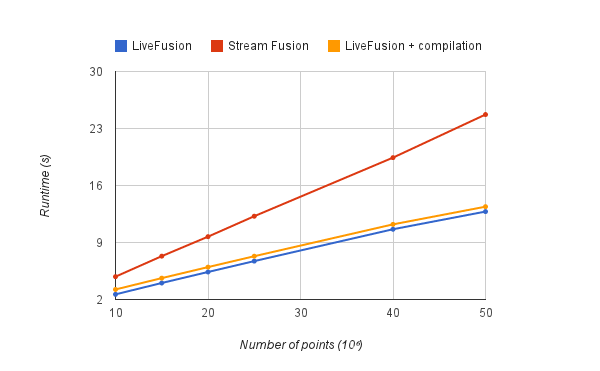
\includegraphics[center]{img/Eval-QuickHull}
\end{figure}

\begin{figure}
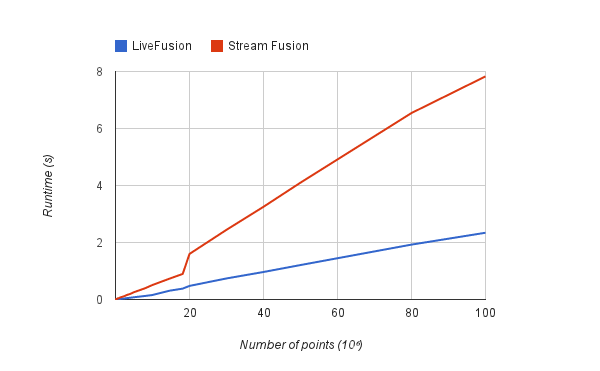
\includegraphics[center]{img/Eval-FarAndAboves}
\end{figure}

\begin{figure}
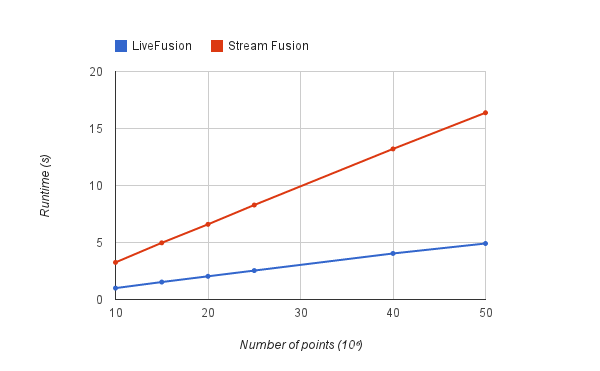
\includegraphics[center]{img/Eval-FarAndAboves-Overall}
\end{figure}

\clearpage
\section{Compilation time and amortisation}


\IfNotCompilingAll{\bibliography{bib}}

\end{document}